\section{Methodology}\label{sec:methodology}

All experiments concerning the data collection and processing were performed at the long-wavelength MX beamline I23 at Diamond Light Source, UK. The data collection takes two experimental modes: X-ray diffraction and X-ray tomography. Data processing was also carried out at beamline facilities. %data from crystal samples at the I23 endstation.

\subsection{Diffraction and tomography data collection}

Experiments detailed in this project were collected on protein crystals of: thaumatin, thermolysin (x2), insulin, and proteinase-K. Additional crystals listed in the appendix include chlorite dismutase (Cld) and OmpK36.
Sample preparation for in-vacuum data collection followed the standard procedure for I23 detailed by Duman \textit{et al.} (2021) \cite{Duman2021}.

The in-vacuum sample environment contains a cylindrical P12M detector as well as a multi-axis goniometer to enable collection  in multiple orientations; this provides access to high multiplicity in addition to just high repetition, which improves data completeness \cite{Finke2016}. The axes of orientation are a kappa and phi angle. %(illustrated PICTURE)

Each diffraction experiments carried out on the protein crystals in this study collected a full set of data, meaning that 360$\degree$ of data was collected. The diffraction data was automatically integrated with DIALS which provides the raw intensities, incident vectors, scattering vectors, and goniometer angles.

Following a diffraction experiment, the sample is kept in its in-beam position while the tomography camera is moved out of its retracted position to immediately start tomography collection. The order of the experiments is important because radiation damage will affect the higher resolution information first. A tomography camera is integrated into the sample environment to allow for a simple transition between the experimental modes \cite{Kazantsev2021}, as seen in \cref{fig:vacuum_chamber}.

\begin{figure}
    \centering
    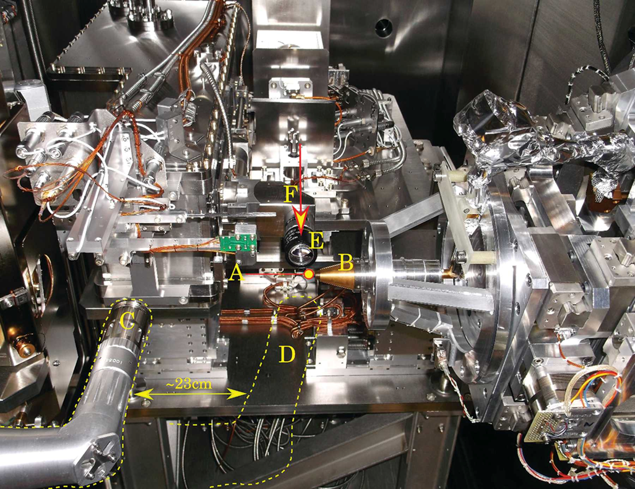
\includegraphics{images/tomo camera.png}
    \caption{A: Sample position; B: goniometer; C: tomography camera in retracted position; D: tomography camera in-beam position; E: viewing system; F: X-ray beam direction. Produced by Kazantsev \textit{et al.} (2021) \cite{Kazantsev2021}.}
    \label{fig:vacuum_chamber}
\end{figure}

Diffraction collection require the user to specify the wavelength, rotation increment, and beam transmission. Likewise, the positioning of the goniometer needs to be closely surveyed to match the chosen kappa and phi angles, which also must be specified by the user for each collection. The relevant collection parameters used for each diffraction experiment on the aforementioned crystals can be found in \cref{diffration_table} in the appendix. Tomography collection also requires a specified wavelength, exposure time, 

Further information on the step-by-step procedure of tomography data collection at I23, as used in this work, is detailed in \href{https://confluence.diamond.ac.uk/x/h4HVDQ}{Tomography data collection instructions} on the Diamond Confluence page.

\subsection{Laser-shaping in cryo-crystallography}
% Unibody-Design fs laser
Beamline I23 now houses a commercial femtosecond laser  that has been set up for laser-shaping crystal samples in-cryo. The product by Light Conversion is a \textbf{CARBIDE-CB5-6W} laser, with a tunable pulse duration between 190 \unit{fs} and 20 \unit{ps}, a maximum power output of 6 \unit{W}, and and an air-cooled model. The laser is also installed with the \textbf{2H} \textit{HG for CARBIDE} harmonic generator model by Light Conversion, with an output wavelength of 515 \unit{nm}, mounted on the laser head.
%https://lightcon.com/product/carbide-femtosecond-lasers/#cb5-specifications
%https://lightcon.com/product/harmonic-generator-for-carbide/#specifications

To allow for the swift transfer of samples from a liquid nitrogen bath directly to the air-cooled goniometer set up at the femtosecond laser, the laser room used by I23 also houses \href{https://www.diamond.ac.uk/Home/Corporate-Literature/Annual-Review/Review2015/Villages/Macromolecular-Crystallography-Village/Macromolecular-Crystallography-Village-Developments/BART---the-new-robotic-sample-changer-for-MX-beamlines-at-Diamond.html}{BART}, a robotic sample changer for \ac{mx} beamlines at Diamond. The experimental setup allows for samples to be sustained at cryogenic temperatures entirely while being laser-shaped and during transfer.

\subsection{Data processing pipelines, DIALS, and AnACor}

Following collection, diffraction data was integrated with DIALS for scaling and merging. DIALS is the standard practice data reduction software at Diamond Light Source that uses SH to produce reflection data in the form of an \textit{mtz} file. This likewise calculates the merging statistics that provide information on merged data quality.% $I/ \sigma$ and $R_{merge}$ values.

%Once the merging statistics have been obtained, the reflection data is also produced .
%Further experiments can be run with \href{http://ccp4.github.io/dimple}{Dimple}, an MX pipeline for structure refinement, provided there are anomalous scatterers in the crystal. Using the known \textit{pdb} file of the protein model with the reflection data in an \textit{mtz}, Dimple calculates anomalous density (Anode) peaks from atoms in the structure. The peak heights are affected by several factors, including structural isomerism, binding ions, and water molecules contained in the pdb. While they are not as reliable as merging statistics for assessing the reflection quality, they are used to generate high-resolution electron density maps, as seen in cref{}, which is imperative for MX structure determination.

The alternative to DIALS in generating reflection data is taken using X-ray tomography, which is a longer, multi-step process as it currently entails manually reconstructing the sample model.

Tomography data can be visualised in ImageJ or in DAWN. After the completion of every tomography scan, the data would be processed using the SAVU pipeline \cite{Kazantsev2022}. The processing routine here first required determination of the centre of rotation to align the tomography images; after this was a flat-field correction, followed by ring-artefact removal and reconstruction. Images were also cropped according to necessity to remove as much background as possible. The final output from SAVU provides two types of reconstructed images: the flat fields (face-on view of the sample), and the tomography slices (stacked along the long axis of the sample). Examples of the flat-field images, raw projections, and flat-field corrected projections are shown in \cref{fig:tomo projections}.

\begin{figure}
    \centering
    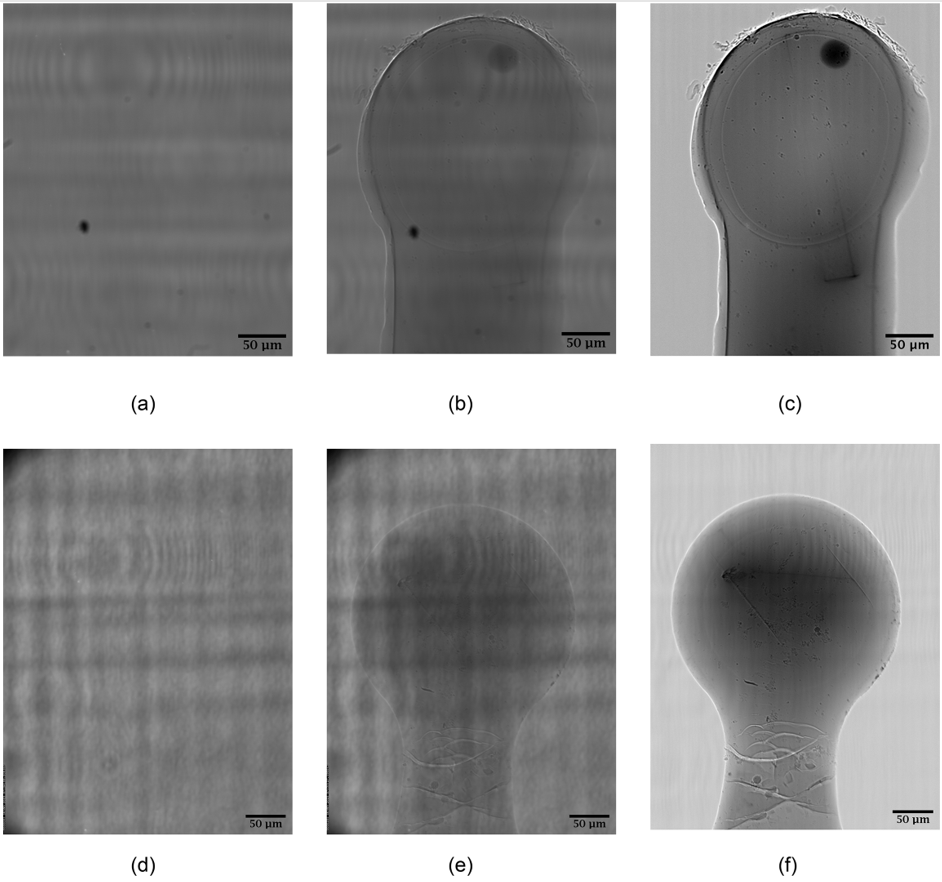
\includegraphics[width = 0.5\textwidth]{images/Tomo projection images CLD and Ompk high quality.png}
    \caption{Tomography projection images of Ompk (top row) and Cld (bottom row) showing: ((a) and (d)) background,  ((b) and (e)) sample, and ((c) and (f)) flat-field corrected images. Produced by Lu \textit{et al.} (Unpublished) \cite{Lu}.}
    \label{fig:tomo projections}
\end{figure}

Following reconstruction in SAVU, the tomography images in the form of 32-bit two-dimensional tiff files were converted to 8-bit data to reduce the data size. The 8-bit data was then imported and manually segmented in the visualisation software Avizo (Thermo Fisher) to distinguish between the different materials. The segmentation annotates every voxel in each tomography slice to a sample material or to the background, which in turn produces a detailed 3D sample model.

%\begin{figure}
    %\centering
    %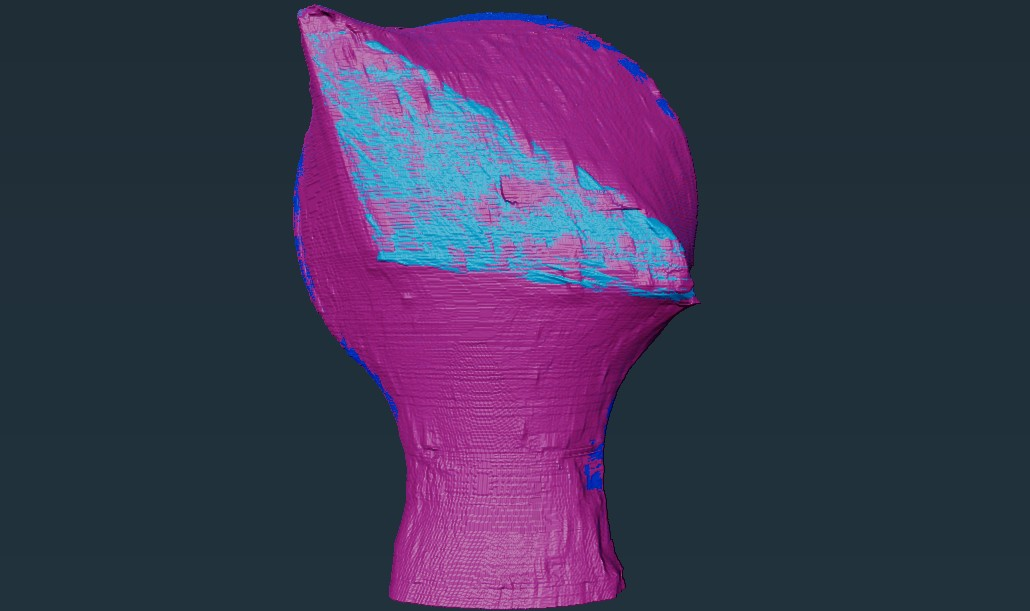
\includegraphics[width = 0.9\textwidth]{images/avizo_flats/cas3_1118.jpg}
    %\caption{3D-segmented model of cryopreserved sample of Cas3 crystal rendered in Avizo; the present materials are crystal (light blue), mother liquor (pink), sample mount (dark blue).}
    %\label{fig:Avizo}
%\end{figure}

The final step to tomography processing is done in AnACor, a ray-tracing software that has been developed collaboratively between I23, Graeme Winter at Diamond Light Source, and Yishun Lu at the Department of Engineering, University of Oxford. AnACor calculates the absorption factors for materials in an analytical 3D model with a discrete form of \cref{AbsFactor}, where the integral over crystal elements $dV$ is replaced with a sum over the crystal voxels $\Delta V$ from  reconstruction \cite{Lu}: %applies an analytical absorption correction strategy based on the 3D model of the sample derived from X-ray tomography.

\begin{equation}
    A_{\hkl} = \frac{1}{N} \sum_{n=1}^N A_{\hkl}^{(n)}
\end{equation}
% which visualises provisional 3D models
AnACor runs in two stages: pre-processing and post-processing. In the pre-processing stage, the user collects the 3D-segmentation labels exported from Avizo and the cropped flat-field images, and feeds these into AnACor to produce a threshold of the sample highlighting where it has high confidence in the presence of a certain percentage of each material. The outcome of pre-processing is a list of absorption factors that are based on where it believes 25\%, 50\%, 75\%, and 100\% of each material lies - this is known as the acceptance percentage. A lower acceptance percentage corresponds to higher confidence, and vice versa. % acceptance of the presence

Absorption factors used in the AnACor experiments were based on 50 \% acceptance of the material, unless stated otherwise.

In the post-processing stage, an absorption factor is chosen for each material, presumably from the list produced in pre-processing. By default, AnACor autofills these with 50 \% acceptance, as this tends to be the optimal percentage covering the largest area without risking overestimation of material presence. Post-processing also requires the reflection data generated by DIALS. For this reason, the reflection data must be initially produced with DIALS prior to running AnACor. In post-processing, the user can set \textit{anomalous difference} to true or false, depending on whether there is believed to be anomalous scattering. The outcome of this stage is the same as in DIALS; reflection data, along with data statistics on merging quality - the difference to DIALS is that the two sets of reflection data produced have been corrected analytically; one with \ac{sh} applied and one without.

Because pre-processing does not generate new reflection data and instead only calculates experimental absorption factors, the first stage of the software can also run on samples void of diffracting material, such as an empty loop or a loop containing solvent. The advantage of this is that samples containing only or largely one type of material will produce more reliable coefficients. The outputted values for the non-diffracting materials can then be used in the post-processing of another sample containing the same kind of solvent or loop, as well as the crystal.

Information on the AnACor ray-tracing algorithm applied to tomographic reconstructions is described in further detail in Lu \textit{et al.} \cite{Lu}.

Subsequent processing after obtaining reflection data is run with \href{http://ccp4.github.io/dimple}{Dimple}, an MX pipeline for structure refinement, provided there were anomalous scatterers of interest in the crystal. Using the known \textit{pdb} file of the protein model with the reflection data in an \textit{mtz}, Dimple calculates anomalous density (Anode) peaks from atoms in the structure. The peak heights are affected by several factors, including structural isomerism, binding ions, and water molecules contained in the pdb. While the peaks are not as reliable as merging statistics for assessing the reflection quality, Dimple likewise generates high-resolution electron density maps, as seen in cref{}, which are imperative for MX structure determination.

Thorough information detailing the step-by-step procedure of data processing in this work, from collection to running Dimple, can be found on Diamond Confluence: \href{https://confluence.diamond.ac.uk/x/yIWuD}{Tomography data processing instructions}. %summarised in cref{}

%\subsection{Phenix $f"$-refinement for ion identification}

\subsection{Merging statistics: R factor, intensities and estimated uncertainties}

In diffraction experiments, the data quality is usually assessed by the global $R_{merge}$ factor based on the reflection intensities. $R_{merge}$ is a measure of the average ratio of the spread of symmetry-equivalent reflection intensities to the estimated value of reflection intensity \cite{Dauter1999}:

\begin{equation}
    R_{merge} = \sum_{\hkl}\sum_i | I_{\hkl,i} - \langle I_{\hkl} \rangle | / \sum_{\hkl} \langle I_{\hkl} \rangle
\end{equation}

The value itself is calculated in different ways across different data reduction programmes. Because it highly depends on data multiplicity, the R factor is always higher for high-symmetry space groups compared to those in low symmetry. Higher multiplicity in turn leads to improved data quality, but this must also be weighed with the increase in the R factor.

The merging of diffraction data naturally increases data multiplicity, which can be appealing for enhancing the quality of crystals of low-symmetry space groups with low multiplicity. As with any experiment, outliers can occur. This can be the result of incorrectly classified partially and fully recorded reflections. Merging equivalent intensities provides a chance to identify outliers and remove them from a diffraction experiment. This however must be done with a level of scrutiny and a physical reason for the rejection.

Complementary information about the data quality is provided by the ratio of intensities to their uncertainties:

\begin{equation}
    I / \sigma = \sum_{\hkl} I_{\hkl}/\sum_{\hkl} \sigma(I_{\hkl})
\end{equation}

Here, the $\sigma$ values are not trivially estimated and are usually computed in data reduction software packages. Correctly estimating intensity uncertainties is crucial for subsequent applications of the data, for instance in phasing, refinement, and the solving of anomalous-atom positions \cite{Dauter1999}.  

It was therefore in the interest of the following experiments to maximise the $I / \sigma$ values while minimising the $R_{merge}$ factors. These were the main parameters used in the assessment of data quality throughout this project.

Two other complementary indicators for assessing diffraction data quality are the resolution and completeness. The data completeness is defined by the number of reflections collected compared to the number of theoretically possible reflections for a given crystal symmetry \cite{Arkhipova2017}. This could range from ... Since each reflection contributes to the electron-density map, the completeness heavily determines the quality of maps \cite{Wlodawer2007}.

